% --------------------------------------------
% Author: Felipe Alfonso González
% https://github.com/felipealfonsog
% f.alfonso@res-ear.ch / felipe.alfonso.glz@gmail.com
% License: MIT / BSD 3-clause License
%
%%%%%%%%%%%%%%%%%%%%%%%%%%%%%%%%%%%%%%%%%

%----------------------------------------------------------------------------------------
%	PACKAGES AND OTHER DOCUMENT CONFIGURATIONS
%----------------------------------------------------------------------------------------

\documentclass[
    a4paper, % Paper size, use either a4paper or letterpaper
    10pt, % Default font size, can also use 11pt or 12pt, although this is not recommended
    unnumberedsections, % Comment to enable section numbering
    twoside, % Two side traditional mode where headers and footers change between odd and even pages, comment this option to make them fixed
]{LTJournalArticle}

\usepackage{amsmath}

\usepackage{hyperref}

\usepackage{amsmath} % amsmath package

\usepackage{graphicx}

\usepackage{comment}

\addbibresource{biblio.bib} % BibLaTeX bibliography file

\runninghead{} % Leave this command empty for no running head

\footertext{} % Leave this command empty for no footer text

\setcounter{page}{1} % The page number of the first page, set this to a higher number if the article is to be part of an issue or larger work

%----------------------------------------------------------------------------------------
%	TITLE SECTION
%----------------------------------------------------------------------------------------

\title{Big Data Marketing}

% Authors are listed in a comma-separated list with superscript numbers indicating affiliations
% \thanks{} is used for any text that should be placed in a footnote on the first page, such as the corresponding author's email, journal acceptance dates, a copyright/license notice, keywords, etc
\author{%
    Felipe Alfonso González\textsuperscript{1}\thanks{Corresponding author: \href{mailto:f.alfonso@res-ear.ch}{f.alfonso@res-ear.ch}}\\
    \textit{ Computer Science Engineer}\\
    \footnotesize Institute of Arts and Communication Sciences (IACC), Chile\\[-6pt]
    \footnotesize Candidate for Master in Big Data, ENEB / Isabel I University\\[-6pt]
    \footnotesize\href{mailto:f.alfonso@res-ear.ch}{f.alfonso@res-ear.ch} - 
    \href{https://glzengrg.com}{glzengrg.com} - 
    Twitter: \href{https://twitter.com/felipealfonsog}{@felipealfonsog} - 
    LinkedIn: \href{https://linkedin.com/in/felipealfonsog}{felipealfonsog}\\
    \scriptsize This manuscript has been authored using the typesetting system \LaTeX{}. \\[-6pt]
    \scriptsize This manuscript is released under the BSD 3-clause License. \\
}


%----------------------------------------------------------------------------------------

% Full-width abstract
\renewcommand{\maketitlehookd}{%
    \begin{abstract}
        \noindent En el entorno altamente competitivo actual, la retención y satisfacción de clientes son imperativos fundamentales. A lo largo de la historia del marketing, se han implementado diversas estrategias para impulsar las ventas y fomentar la lealtad, pero en la actualidad, la personalización se ha vuelto esencial en este contexto de feroz competencia. 
        Este paper explora el marketing desde la perspectiva del big data, destacando cómo las empresas pueden aprovechar los datos disponibles sobre clientes y entorno para diseñar estrategias altamente personalizadas. Ya no es suficiente con promociones genéricas; ahora, la clave radica en ofertas específicas que se alineen con las preferencias individuales de cada cliente. 
        Al reconocer que los clientes son la piedra angular de una empresa, se enfatiza la importancia de planificar acciones y estrategias personalizadas. Estos enfoques no solo aseguran la supervivencia de la empresa en un mercado dinámico, sino que también generan lealtad y fidelidad del cliente, aportando un valor significativo al negocio. 
        
    \end{abstract}
}

%----------------------------------------------------------------------------------------



\begin{document}

\maketitle % Output the title section

%----------------------------------------------------------------------------------------
%    PAPER CONTENTS
%----------------------------------------------------------------------------------------

\section{Introduction}

En el panorama empresarial actual, marcado por una competencia feroz, la retención de clientes y su satisfacción plena se presentan como objetivos cruciales para la supervivencia y el éxito de cualquier empresa. A lo largo de la historia, el marketing ha evolucionado desde estrategias generales hasta reconocer la necesidad de personalización en un mundo donde cada cliente es único. Este paper aborda el desafío de implementar estrategias de marketing desde la perspectiva del big data, explorando cómo la información sobre clientes y su entorno puede ser aprovechada para diseñar ofertas altamente específicas. En un contexto donde los clientes son la esencia misma de la empresa, este enfoque personalizado no solo asegura la permanencia en el mercado, sino que también cultiva la lealtad y la conexión duradera con la clientela, generando un valor distintivo para el negocio. \cite{ENEB2023}.

\subsection{El Marketing: necesidades, deseos y demandas}

Todas las personas pueden tener diferentes tipos de necesidades, que son parte de la esencia humana y pueden ser físicas (como alimentarse), seguridad, o sociales o individuales; pero sus deseos pueden estar alineados con sus necesidades, que pueden ser físicas, como alimentarse o sentirse seguro, o algún tipo de realización personal, entre otras. Pueden variedad según incluso por cuan importantes deseas sentirse. En relación a las demandas, son los deseos, y estas se convierten en demanda cuando existe esa capacidad adquisitiva. 

El ser humano, satisfaces sus necesidades con productos y servicios. Pueden ser estos intangibles como los servicios en algún área, o tangibles. Pueden ser susceptibles a algo que puede ser ofrecido para satisfacer necesidades y deseos. 


 Todos los consumidores toman decisiones basadas en expectativas que les plantean las diferentes ofertas. Las expectativas de valor que les plantean en las diferentes ofertas. 
 
Los consumidores eligen productos según las expectativas netas de valor, la diferencia entre aspectos positivos y negativos esperados. Este valor impacta en la satisfacción del cliente y su comportamiento futuro, al comparar expectativas con la experiencia real de compra.

El marketing surge del intercambio, un proceso donde las personas satisfacen necesidades a través de ofrecer algo a cambio de dinero, bienes o servicios. Para que el intercambio ocurra, deben existir al menos dos partes con algo de valor para la otra, capacidad de comunicación, libertad de aceptar o rechazar la oferta, y la creencia de que es apropiado tratar con la otra parte. El intercambio es un proceso continuo, y cuando se llega a un acuerdo, se denomina transacción. El marketing de relaciones busca construir relaciones duraderas basadas en confianza mediante la entrega consistente de productos de calidad, buen servicio y precios razonables.


Un mercado es el conjunto de consumidores que comparten una necesidad o deseo y están dispuestos a intercambiar elementos de valor. Su tamaño depende del número de personas con la necesidad específica, recursos atractivos para otros, y la disposición de intercambiar.

El marketing se centra en actividades relacionadas con los mercados para facilitar intercambios potenciales que satisfacen necesidades y deseos. En este proceso, participan dos partes: el buscador de intercambios, usualmente una empresa compitiendo en un mercado, y el receptor. La eficacia del buscador se ve afectada por factores del entorno como demografía, economía, tecnología y aspectos socio-culturales.

%%  Inserting image 
\begin{figure}[h]
  \centering
  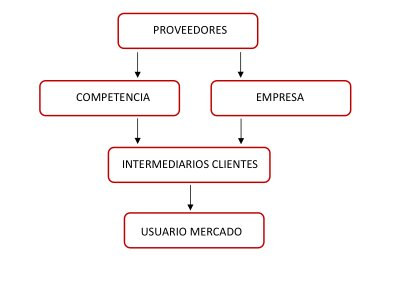
\includegraphics[width=0.7\linewidth]{./images/graph-mkt.jpg}
  \caption{Partes que confirman el marketing}
  \label{fig:etiqueta}
\end{figure}
%% End insert image 


\subsection{Gestión del marketing}

La gestión de marketing se ocupa de planificar y ejecutar estrategias para productos, precios, promoción y distribución, con el objetivo de crear intercambios que satisfagan tanto objetivos individuales como organizativos. Se enfoca en la gestión de la demanda, influenciando su nivel, momento y composición para alcanzar metas organizativas. En un entorno empresarial, la gestión de la demanda busca ajustarse a períodos variables, controlando la oferta para mantenerla alineada con las expectativas del mercado.

Esta gestión no solo trata con la demanda sino también con los clientes actuales, nuevos y potenciales. A lo largo del tiempo, ha evolucionado hacia la creación de relaciones a largo plazo con los clientes, especialmente en la era del big data marketing. La retención y fidelización de clientes son fundamentales en la actual competencia empresarial, lo que destaca la importancia del trato personalizado y la prevención de la pérdida de clientes.

La adquisición de nuevos clientes se considera costosa, siendo aproximadamente cinco veces más costoso que mantener a un cliente existente satisfecho. Además, la pérdida de un cliente habitual puede tener repercusiones más amplias, ya que la insatisfacción puede propagarse a través de redes sociales, afectando la imagen de la empresa.

En relación con las orientaciones empresariales, existen cinco enfoques: producción, producto, ventas, marketing y marketing social. Cada enfoque refleja la filosofía y los intereses que guían a las organizaciones en su desarrollo empresarial. Estos aspectos son fundamentales en la planificación estratégica y el proceso de marketing.


\subsection{Enfoque de producción}

El enfoque de producción masiva es el más antiguo en la dirección de intercambios, priorizando la disponibilidad y el bajo costo de los productos. Se centra en alcanzar economías de escala y una amplia distribución, con énfasis en la producción en lugar de la creación de clientes. Predomina en situaciones donde la demanda supera la oferta, como en países del tercer mundo, o cuando se busca reducir costos para ampliar el mercado. Un ejemplo destacado es el enfoque de producción masiva y precios bajos de Henry Ford en 1900, que perfeccionó la producción de automóviles para hacerlos más accesibles a la población. En resumen, implica producir en gran cantidad para lograr costos bajos y precios de venta asequibles.


\subsection{Enfoque de producto}

El segundo enfoque destaca la importancia de ofrecer productos de alta calidad o con resultados superiores para atraer a los consumidores. Implica esfuerzos constantes en la fabricación de productos de excelencia y su mejora continua. Los directores de empresas que siguen este enfoque creen que los compradores valoran la calidad del producto, centrándose en las ventajas y beneficios. Sin embargo, puede haber descuidos en la atención al mercado y la comprensión de la demanda, llevando a la miopía de marketing. Esto podría resultar en productos que no cumplen con las expectativas y carecen de utilidad. Equilibrar la calidad del producto con una comprensión profunda del mercado es crucial para el éxito sostenible de la empresa.



\subsection{Enfoque de ventas}

El enfoque de ventas se centra exclusivamente en impulsar las ventas mediante estrategias agresivas de venta y promoción. Su objetivo principal es vender la mayor cantidad posible de productos, priorizando la venta de lo que se produce en lugar de producir según la demanda. Este enfoque se utiliza principalmente para bienes no buscados, aquellos que los consumidores no tienen la intención de adquirir habitualmente. Sin embargo, también se aplica a productos buscados o de áreas no lucrativas.

Este enfoque también es comúnmente empleado por las empresas cuando tienen capacidad productiva excedente y buscan liquidar el stock disponible.

\subsection{Enfoque de marketing}

El enfoque de marketing se diferencia de los anteriores al poner énfasis en identificar las necesidades y deseos de los clientes para satisfacerlos efectivamente. En este enfoque:

- Se centra en las necesidades del comprador.
- Busca satisfacer las necesidades del cliente a través del producto y los beneficios asociados con su entrega y consumo.

Este enfoque se fundamenta en cuatro pilares esenciales: definición del mercado, orientación al cliente, coordinación de marketing y rentabilidad.



\section{Definición del mercado}

Cada empresa debe cuidadosamente definir su público objetivo, ya que es imposible operar en todos los mercados y satisfacer todas las necesidades. La elección del público objetivo influye en las acciones que la empresa emprenderá para satisfacer las necesidades de ese grupo específico. Por ejemplo, una empresa de viajes organizados debe determinar con precisión el tipo de cliente al que se dirige, ya que esto condicionará el producto y la presentación del mismo. La planificación de viajes de lujo para recién casados difiere significativamente de organizar viajes de fin de curso para universitarios o viajes del IMSERSO.


\section{Orientación al cliente}

Una vez definido el público objetivo, es esencial comprender sus necesidades desde su perspectiva, no desde la de la empresa. Esto implica identificar cinco tipos de necesidades:

Necesidades declaradas: El cliente desea un coche asequible.
Necesidades reales: El cliente busca un coche con bajos costos operativos, no solo un precio de compra bajo.
Necesidades no declaradas: El cliente desea recibir un buen trato y servicio de la empresa vendedora.
Necesidades de deleite: El cliente recibe regalos o servicios adicionales con la compra del coche.
Necesidades secretas: El cliente quiere ser percibido como alguien que obtiene un buen valor por su dinero.
Para satisfacer estas necesidades, el departamento de marketing debe investigar los aspectos más valorados por el público objetivo. El objetivo principal es vender a través de la satisfacción del cliente, ya que un cliente satisfecho:

Compra repetidamente y es leal.
Adquiere nuevos productos lanzados por la empresa.
Habla positivamente sobre la empresa y sus productos.
Presta menos atención a las marcas y publicidad de competidores.
Es más rentable de servir debido al conocimiento detallado sobre sus preferencias.
Contribuye con ideas para nuevos productos y servicios.
La satisfacción del cliente es crucial, ya que un cliente insatisfecho puede dañar la reputación de la empresa. Medir regularmente el grado de satisfacción, incluyendo quejas y reclamaciones, es vital para la mejora continua.



\section{Coordinación de marketing}

El éxito de una empresa depende crucialmente de la coordinación. En el ámbito de la coordinación de marketing, dos aspectos fundamentales deben ser considerados:

Coordinación de funciones de marketing: Es esencial que las diversas funciones de marketing, como ventas, publicidad, gestión de productos, investigación, entre otras, trabajen de manera conjunta y coordinada desde la perspectiva del consumidor. Este enfoque busca lograr la plena satisfacción de los clientes.

Coordinación del departamento de marketing con el resto de la empresa: El departamento de marketing no puede operar de manera aislada; debe estar coordinado con otros departamentos de la empresa. La falta de coordinación interna dificulta la plena satisfacción de los clientes.

La empresa debe llevar a cabo tanto acciones de marketing externo como interno. El marketing interno se refiere a la contratación, capacitación y motivación del personal para que brinde un servicio adecuado a los clientes. Es crucial reconocer que el marketing interno precede al marketing externo; prometer un excelente servicio a los clientes carece de significado si internamente la empresa no está preparada para cumplir con esas promesas.



\section{Rentabilidad}

La rentabilidad es un objetivo clave del enfoque de marketing, buscando contribuir a que las organizaciones alcancen sus metas, generalmente centradas en maximizar beneficios. Por lo tanto, el departamento de marketing no solo trabaja para satisfacer a los clientes, sino también para lograr rentabilidad.


\subsection{Enfoque de marketing social}

El enfoque de marketing social va más allá de la satisfacción del cliente y la rentabilidad, considerando también el impacto en la sociedad y el interés público en la toma de decisiones. La Responsabilidad Social Corporativa (RSC) es esencial en este enfoque, gestionando los impactos de la actividad empresarial en clientes, empleados, accionistas, medio ambiente y la sociedad en general.

La RSC equilibra el crecimiento económico, el bienestar social y la sostenibilidad ambiental. Esto no solo beneficia a la sociedad, sino que también aporta ventajas para la empresa, como mayor productividad, lealtad del cliente, acceso a mercados y credibilidad. La transparencia y la adaptabilidad a las expectativas de la sociedad son clave para lograr la responsabilidad social y el éxito a largo plazo.

El marketing social no solo busca beneficios para la empresa y los clientes, sino también para la sociedad y el entorno. Se destaca la importancia de la adaptación al mercado y a las necesidades de los diferentes grupos de interés. En este contexto, el big data marketing surge como una evolución del marketing tradicional, proporcionando herramientas avanzadas para comprender y abordar las complejidades del mercado actual.



\section{Big Data Marketing}

El big data marketing se centra en aprovechar la gran cantidad de datos disponibles sobre clientes para personalizar estrategias y promociones de manera individualizada, evitando campañas genéricas. A diferencia de la segmentación tradicional, el enfoque del big data marketing se dirige exclusivamente a un cliente concreto.

Los elementos clave para trabajar con éxito el big data marketing son:

Tener una estrategia: Es esencial definir qué tipo de cliente se desea abordar y cómo llevar a cabo la interacción. Esto implica establecer una estrategia de interacción y definir la estrategia analítica, determinando qué datos son relevantes para el negocio.

Personalización, relevancia y recompensa: Implementar un sistema de big data conlleva un alto costo, por lo que es crucial utilizar el conocimiento del cliente para personalizar ofertas y comunicaciones, identificar clientes clave y recompensarlos según el valor que aportan.

En el big data marketing, el cliente se convierte en el protagonista principal, y se debe adaptar el marketing al ciclo de vida del cliente. El customer analytics, herramienta utilizada para analizar datos de clientes, se vuelve crítico en este entorno de alto conocimiento del cliente.

El ciclo de vida del cliente consta de seis fases:

Descubrir: Conocer la marca.
Explorar: Evaluar si gusta.
Comprar
Usar
Preguntar
Ser un fan: Convertirse en un cliente de alto valor.
La gestión efectiva de este ciclo de vida implica que un cliente que descubre y explora la marca llegue a comprar y convertirse en un fan. Cada fase tiene objetivos de negocio específicos y requiere métodos analíticos particulares para su gestión óptima.


%%  Inserting image 
\begin{figure}[h]
  \centering
  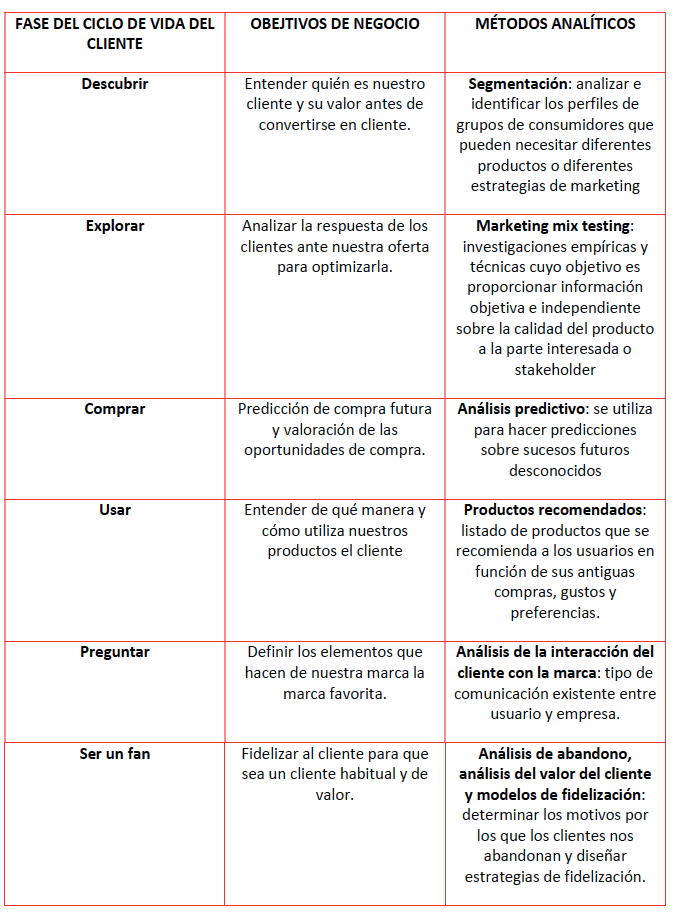
\includegraphics[width=0.7\linewidth]{./images/bgmkt.jpg}
  \caption{Fases, métodos y objetivos del Big Data Marketing}
  \label{fig:etiqueta}
\end{figure}
%% End insert image 


En el contexto de la gestión de clientes mediante el big data marketing, es fundamental considerar el concepto de "customer journey" o viaje del cliente, que se analiza en el módulo de Customer Analytics. Este enfoque implica mapear las etapas, interacciones, canales y elementos por los cuales se desplaza el cliente dentro de la empresa. El customer journey no se limita a la etapa de cliente hasta su finalización; puede centrarse en un punto específico, como el proceso de compra o la atención al cliente para resolver un problema.

Al construir estos mapas, se deben tener en cuenta varios aspectos:

Identificación del cliente: Es esencial conocer y entender al cliente desde su perspectiva.

Comprensión de las etapas del vínculo: Observar cómo se siente el cliente en cada interacción con la empresa, servicio o producto.

Registro de indecisiones y motivaciones: Conocer lo que motiva a los consumidores y sus inquietudes.

Mapeo de interacciones: Identificar los puntos de contacto repetitivos en las relaciones con la empresa.

Análisis de instancias clave: Detectar momentos cruciales en los que el cliente se siente feliz, enojado o perdido, ya que impactan en la decisión de avanzar o abandonar.

Procesos internos de la empresa: Opcionalmente, agregar procesos internos de la empresa relacionados con cada interacción del cliente para entender cómo contribuyen a la experiencia.

Oportunidades y sentimientos: Comprender las sensaciones y sentimientos del cliente en cada etapa o interacción, especialmente identificar lo que le molesta o incomoda.

Trazar este viaje ayuda a comprender mejor las motivaciones y la satisfacción del cliente, facilitando una gestión personalizada que guía al cliente a través de todas las fases del ciclo de vida. Esto solo se logra mediante un análisis detallado del cliente y la implementación de acciones de marketing personalizadas basadas en los resultados del análisis.

El big data marketing representa un cambio significativo en las relaciones con los clientes, pasando de una comunicación masiva a una personalizada que se adapta a las necesidades individuales de cada cliente. Aunque la segmentación sigue siendo importante, la personalización adquiere una relevancia aún mayor.

Estas consideraciones preparan el terreno para explorar las herramientas esenciales en el ámbito del big data marketing.



\subsection{Herramientas y prácticas de big data marketing}


Para implementar con éxito el big data marketing, es crucial emplear diversas herramientas además del análisis de clientes. Estas herramientas incluyen:

Email Marketing: Esta estrategia se centra en el uso efectivo del correo electrónico como medio para comunicarse con los clientes. Permite enviar mensajes personalizados, campañas específicas y promociones adaptadas a las necesidades individuales de cada cliente. El email marketing es una herramienta clave para establecer y mantener una conexión directa y personalizada.

Mobile Marketing: El mobile marketing se enfoca en llegar a los usuarios a través de dispositivos móviles, como teléfonos inteligentes y tabletas. Con el auge de los dispositivos móviles, esta herramienta se vuelve esencial para llegar a los clientes dondequiera que estén. Incluye estrategias como mensajes de texto, aplicaciones móviles y publicidad específica para dispositivos móviles.

Social Marketing: Las redes sociales desempeñan un papel fundamental en el big data marketing. Esta herramienta implica la utilización de plataformas como Facebook, Twitter, Instagram, entre otras, para interactuar con los clientes, conocer sus opiniones y preferencias, y promover productos o servicios de manera personalizada. El social marketing es valioso para construir relaciones sólidas con los clientes y generar interacción directa.

Explorar y comprender estas prácticas es esencial para utilizarlas efectivamente en un enfoque de big data marketing, asegurando así una comunicación personalizada y adaptada a las necesidades individuales de cada cliente.



\subsection{Email marketing}

El email marketing, una herramienta de marketing directo que utiliza el correo electrónico para realizar campañas publicitarias y promocionales, ha ganado gran popularidad con el auge de internet. Se ha convertido en una alternativa más eficiente y económica que las promociones enviadas por correo postal, permitiendo una entrega inmediata y la medición de resultados.

Aunque pueda parecer simple, una estrategia de email marketing requiere una planificación cuidadosa y el seguimiento de varios procesos en tres fases clave:

Planificación:

Fijar objetivos a corto, medio y largo plazo.
Objetivos comunes incluyen branding, transacciones, captación y cualificación.
Ejecución:

Definir el público objetivo.
Determinar el mensaje y la acción deseada del consumidor.
Establecer el momento de envío.
Medición de Resultados:

Evaluar métricas como entregabilidad, apertura, click y conversión.
Obtener conocimiento adicional sobre los clientes para futuras campañas.
En el contexto del big data y el customer analytics, el email marketing se beneficia de:

Target de envío:
Utilizar datos del big data para conocer mejor a los clientes y definir un target de envío específico.
Evitar envíos masivos y enviar correos solo a clientes potencialmente interesados.
Personalizar estrategias con micro-segmentos, permitiendo una comunicación más detallada y dirigida.
La integración de big data y customer analytics ha llevado a una estrategia más refinada de email marketing, asegurando que los mensajes se envíen a las personas adecuadas y contribuyendo a relaciones duraderas con los clientes.



\subsection{Personalización del contenido}

La micro-segmentación facilita la presentación de contenidos altamente diferenciados para cada tipo de cliente, permitiendo una comunicación más precisa y efectiva. Aunque esta estrategia puede excluir a una parte de la base de datos, se contrarresta con la personalización del contenido.

Personalización del Contenido:

Ventaja: Contenidos exclusivos para cada cliente, percibidos como más valiosos, mejorando resultados a corto, medio y largo plazo.
Desventaja: Mayor personalización implica más recursos.
La decisión sobre el nivel de personalización debe equilibrar los beneficios y costos asociados. La personalización adicional debe ser económicamente rentable, donde los beneficios superen los costos, llegando a un compromiso entre la calidad del mensaje y los recursos invertidos.


\subsection{Momento y frecuencia de envío}


El éxito de la campaña depende del momento en que el email aparece en la bandeja de entrada del receptor.
Una cuarta parte de los emails se abre en la primera hora de recepción, y esta tasa disminuye significativamente después de 24 horas.
Principios Básicos para el Envío:

Evitar envíos durante la franja nocturna.
Evitar los martes para evitar competir con correos acumulados durante el fin de semana.
Estadísticamente, el mejor día y franja horaria son jueves de 8 a 9 de la mañana, seguido de miércoles de 8 a 10.
Adaptación con Big Data:

Gracias al análisis detallado del big data, se puede definir el mejor momento de envío.
Pautas para adaptar el momento de envío:
Conocer el mejor día de envío por usuario.
Crear una variable de frecuencia de apertura a nivel de usuario para determinar la frecuencia de envío por usuario.



\subsection{Puesta en escena}

Tipos de Emails y Captación de Datos en Email Marketing:

Emails Transaccionales:

Orientados a generar ventas.
Utilización del big data para determinar productos de interés, preferencias de ofertas y estrategias para aumentar el ticket medio.
Enfocados en aumentar las ventas.
Emails de Marca:

Personalizados para comunicar lo que interesa al cliente sobre la marca.
Contribuyen a construir una imagen positiva y reputación.
Captación de Datos:

Además de vender y mejorar la imagen de marca, los emails deben recoger datos útiles para futuras campañas.
Se busca identificar los posibles clics del receptor para obtener información valiosa.
Categorizar los clics por variables (por ejemplo, categoría o tipo de acción) facilita el análisis.
Ejemplo: Una marca de ropa envía un correo con secciones de ropa para mujer, hombre, hogar y niños durante rebajas. Analizar los clics permite determinar las preferencias específicas del cliente y personalizar futuros correos.


%%  Inserting image 
\begin{figure}[h]
  \centering
  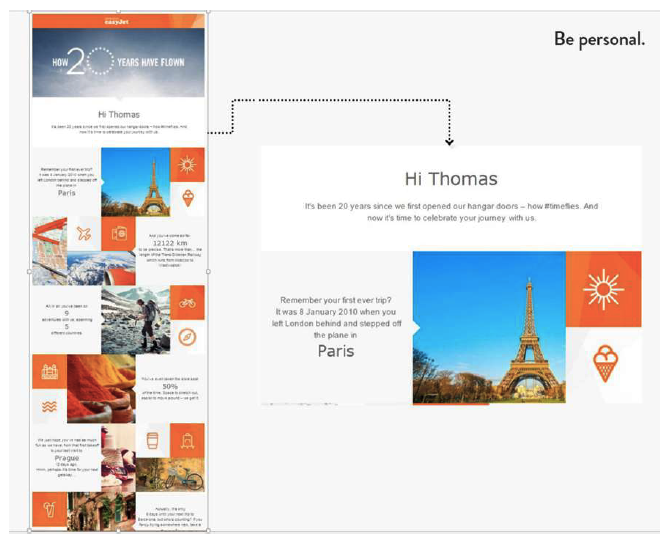
\includegraphics[width=0.7\linewidth]{./images/ex-mailmkt.jpg}
  \caption{Ej. Email marketing}
  \label{fig:etiqueta}
\end{figure}
%% End insert image 



\subsection{Mobile marketing}

Mobile Marketing en Big Data:

El Mobile Marketing en el contexto del Big Data se define como la práctica que permite a las empresas interactuar y conectar de manera relevante con los clientes a través de dispositivos móviles, que incluyen teléfonos móviles y tabletas. Distinguiéndose del marketing tradicional, el mobile marketing aprovecha diversas capacidades de los dispositivos móviles:

Localización: Utiliza sistemas GPS para conocer la ubicación geográfica de los clientes, permitiendo la presentación de anuncios, contenido relevante, o promociones específicas según la localización.

Proximidad: Los dispositivos móviles ofrecen accesibilidad con un solo clic a través de diversas tecnologías.

Aplicaciones: El uso de aplicaciones permite mostrar catálogos de productos y servicios, facilitando a los clientes adquirir productos desde cualquier lugar.

Anuncios para Móviles: Originados en banners tradicionales, estos anuncios se presentan al usuario mientras consume contenido móvil y están relacionados con sus preferencias. Pueden ser formatos de vídeo interactivos.

SMS y MMS: Aunque ha perdido popularidad, los mensajes de texto ofrecen una manera rápida y directa de transmitir información a los clientes, a menudo utilizados como complemento para campañas multicanal.

Cupones Electrónicos: Cupones de descuento electrónicos atraen clientes a las tiendas y eliminan la necesidad de llevar cupones físicos.

Búsquedas Móviles: Los resultados de búsqueda móvil están adaptados a la experiencia de uso móvil, requiriendo estrategias de SEO móvil para la promoción de contenidos dirigidos a usuarios móviles.

En el ámbito del Big Data, el Mobile Marketing se ve potenciado, ya que los dispositivos móviles generan una gran cantidad de datos, proporcionando información valiosa sobre los usuarios. Estos dispositivos permiten a los usuarios permanecer conectados durante todo el día, lo que facilita la recopilación de datos sobre sus comportamientos y preferencias.

La aplicación del Big Data al Mobile Marketing permite la comunicación no solo con el contenido más adecuado sino también en el momento oportuno para cada cliente. La geolocalización y el análisis de datos en tiempo real posibilitan campañas de marketing cercanas y específicas para el público objetivo.

Las principales campañas de Mobile Marketing en Big Data incluyen aplicaciones, comunicación móvil y mensajes personalizados.


Ejemplo de Mobile Marketing: Starbucks y Spotify

Un destacado ejemplo de Mobile Marketing se materializa a través de la colaboración entre Starbucks y Spotify. En esta campaña, los clientes registrados en la aplicación de Starbucks tienen la oportunidad de acceder a listas de música diseñadas exclusivamente para ellos.

Esta iniciativa ilustra cómo las empresas pueden aprovechar las capacidades de las aplicaciones móviles para proporcionar experiencias personalizadas a sus clientes. Al vincular la aplicación de Starbucks con Spotify, se crea un canal único para ofrecer contenido musical que se adapta a los gustos individuales de los usuarios.

El valor añadido radica en la exclusividad de estas listas de reproducción, lo que fomenta la lealtad del cliente. Al proporcionar algo único y personalizado a través de la aplicación móvil, Starbucks no solo mejora la experiencia del cliente sino que también establece una conexión más profunda con su base de consumidores.

Este ejemplo destaca cómo el Mobile Marketing no se trata solo de promociones y anuncios, sino de ofrecer contenido relevante y personalizado a través de dispositivos móviles, aprovechando las capacidades del análisis de datos para entender y satisfacer las preferencias individuales de los usuarios. La colaboración con plataformas populares, como Spotify en este caso, también puede aumentar la visibilidad y el atractivo de la campaña.



%%  Inserting image 
\begin{figure}[h]
  \centering
  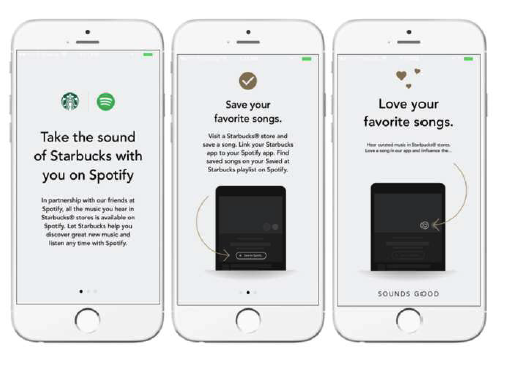
\includegraphics[width=0.7\linewidth]{./images/spostar.jpg}
  \caption{Ej. Campaña Spotify / Starbucks}
  \label{fig:etiqueta}
\end{figure}
%% End insert image 


\subsection{Social marketing}

El Social Marketing, como parte integral del Big Data Marketing, se define como la técnica que utiliza los medios sociales e influenciadores para abordar las necesidades de marketing y negocio de una empresa. Dentro de esta modalidad, se pueden llevar a cabo acciones tradicionales como patrocinios y anuncios sociales, así como estrategias más innovadoras centradas en el marketing de influencias y acciones en redes sociales y blogs de la empresa.

En la relación con el Big Data, los medios sociales son una fuente valiosa de datos no estructurados sobre los clientes, contribuyendo significativamente al diseño personalizado de estrategias de marketing. Los medios sociales no solo ofrecen un canal para la promoción, sino que también proporcionan información detallada sobre las preferencias, comportamientos y opiniones de los usuarios.

Al explorar los medios sociales más populares, se destaca la importancia del contenido generado por los usuarios. Analizar las publicaciones, interacciones y la audiencia de los usuarios en estos medios ofrece una visión profunda del comportamiento del consumidor. Además, aspectos como las visitas, likes, comentarios, comparticiones y el número de seguidores de los usuarios amplían la comprensión del perfil del cliente.

Blogs y Redes Sociales:

Blogs: Estos siguen siendo una plataforma relevante para el Social Marketing. La creación de contenido atractivo y la participación en la blogosfera pueden proporcionar datos valiosos sobre las preferencias de los consumidores.

Redes Sociales: Son un componente esencial, con plataformas como Facebook, Twitter e Instagram que dominan el panorama. La interacción social, los comentarios, los "me gusta" y las actividades compartidas en estas redes ofrecen una ventana única a la psicografía del cliente.

En este entorno, es crucial no solo considerar el contenido generado, sino también analizar las interacciones y el alcance. La cantidad de datos generados en los medios sociales requiere estrategias efectivas de análisis de datos para extraer información significativa y aplicarla en campañas de marketing personalizadas.

En resumen, el Social Marketing en el contexto del Big Data se trata de entender y utilizar la información generada en los medios sociales para construir relaciones más profundas con los clientes y adaptar las estrategias de marketing a sus preferencias y comportamientos específicos.


\subsection{Blogs \& RRSS}

Los blogs son espacios donde empresas o individuos comparten regularmente textos o artículos sobre un tema específico. Aunque algunos consideran que los blogs son innecesarios debido al fuerte impacto de las redes sociales, en realidad, dependiendo del sector, pueden ser recursos valiosos. Los blogs permiten presentar a los usuarios contenido más elaborado que a menudo complementa lo compartido en redes sociales. Aunque plataformas como Facebook o Twitter son útiles para la presentación general, los blogs ofrecen la oportunidad de profundizar en temas específicos de manera más detallada y estructurada.

La estrategia consiste en compartir nuestras novedades a través de las redes sociales, proporcionando enlaces a nuestra web o blog para que los usuarios obtengan información más detallada. Por ejemplo, al entrevistar a alguien influyente en nuestro sector, podemos utilizar Instagram para compartir una foto del entrevistado y dirigir a los seguidores al contenido completo de la entrevista en nuestro blog. Esto asegura que la información se presente de manera atractiva en las redes sociales, pero se redirija a plataformas más amplias y detalladas para una experiencia informativa completa.

\subsection{Las características principales de los blogs incluyen:}


Interactividad Dinámica:

Espacios dinámicos que permiten a los autores interactuar con los usuarios a través de comentarios.
Comunicación Personal e Informal:

A diferencia de los sitios web, los blogs presentan una comunicación más personal e informal, evitando el lenguaje formal y corporativo. Esto crea un medio más cercano para establecer comunicación directa e informal, manteniendo rigor y educación.
Organización Mediante Posts:

Los contenidos se publican a través de posts, clasificados por fecha, categoría y etiquetas para una rápida identificación.
Accesibilidad mediante RSS:

Los blogs pueden ser leídos mediante agregadores de RSS, facilitando la difusión y notificación a los lectores sobre nuevos contenidos publicados.


El microblogging es una forma de publicar contenido mediante mensajes breves, destacando por su simplicidad en la comunicación. Este formato permite transmitir mensajes de manera clara, rápida y precisa debido a las limitaciones de espacio. La naturaleza breve de los mensajes en el microblogging requiere originalidad por parte del emisor para comunicar de manera efectiva en un número reducido de caracteres. Twitter es la plataforma que mejor representa esta forma de comunicación.


% pp 35
\subsection{Redes Sociales: Un análisis mayor}

Las redes sociales son estructuras sociales en las que individuos u organizaciones se relacionan según diversos criterios, como la amistad, el parentesco o relaciones profesionales. En el contexto de Internet, se dividen en tres niveles:

Redes Sociales Genéricas: Son las más comunes, como Facebook, Instagram o Twitter. Su función principal es establecer relaciones entre individuos, ya sea que se conozcan previamente o no. Además, son fuentes de información tanto a nivel personal como público.

Redes Sociales Profesionales: Están orientadas a relaciones profesionales, permitiendo a sus miembros conectar con colegas de trabajo o buscar empleo. Ejemplos notables incluyen Xing o Linkedin.

Redes Sociales Verticales o Temáticas: Están centradas en un tema específico, conectando a usuarios interesados en dicho tema. Ejemplos son Flickr, donde se comparten fotografías de carácter profesional, y Dribble, una red exclusiva para diseñadores gráficos que muestran sus trabajos.



\subsection{Las redes sociales más populares como herramientas valiosas para obtener datos sobre clientes:}

Facebook: Destacado por su popularidad, permite compartir varios tipos de contenido. Se diferencia entre perfiles personales y páginas profesionales. Para empresas, es crucial prestar atención a comentarios, likes, dislikes y contenido compartido.

Twitter: Enfocado en microblogging, es esencial transmitir mensajes atractivos en 280 caracteres. Utilizar hashtags relacionados con la empresa facilita el acceso a comentarios y opiniones sobre la marca.

Instagram: Ideal para contenido visual, permite compartir fotos y videos, incluyendo publicaciones temporales. La red es dinámica y, a través de hashtags, brinda acceso a publicaciones relacionadas con la empresa.

Linkedin: Enfocada en el ámbito profesional, es útil para buscar oportunidades de negocio, establecer alianzas estratégicas y generar una red de contactos. Es eficaz para generar clientes potenciales.

Google+: Aunque menos utilizada, su pertenencia a Google proporciona ventajas en términos de posicionamiento y contacto con usuarios de la plataforma de búsqueda.

Aspectos importantes para obtener datos e información sobre clientes incluyen:

Gestión de Comentarios: Considerar todos los comentarios, tanto positivos como negativos, para evaluar la satisfacción del cliente y mejorar en áreas necesarias.

Comunicación Activa: Mantener una comunicación activa con los clientes a través de comentarios y mensajes privados para construir relaciones sólidas.

Geolocalización: Utilizar la geolocalización para conocer la ubicación física de los clientes y ofrecer servicios personalizados.

Análisis de Contenido: No solo analizar los comentarios sobre la propia marca, sino también estudiar lo que los usuarios comparten sobre otras marcas para obtener una visión más amplia del mercado.

El marketing social basado en datos puede ser de diferentes tipos, como contenido basado en la reacción de los usuarios, publicidad según el perfil del usuario y publicaciones basadas en algoritmos.

Se mencionan herramientas específicas como Facebook Custom Audience y Twitter Custom Audiences, que utilizan datos para acciones de marketing dirigidas, permitiendo a las empresas adaptar mensajes según los criterios definidos por los usuarios. Estas herramientas aprovechan el conocimiento de la base de datos de clientes para la generación de publicidad en redes sociales.


\subsection{Marketing automation}

El marketing automation se refiere a herramientas que automatizan tareas de marketing, especialmente las comunicaciones con usuarios derivadas de acciones específicas. Aunque no todas las acciones comerciales pueden automatizarse, algunas tareas incluyen enviar mensajes de agradecimiento tras una compra, adjuntando información relevante y recomendaciones de productos relacionados. También, se puede personalizar la página de entrada de un e-commerce según la navegación y compras de los usuarios, adaptando la experiencia a sus intereses y preferencias. La automatización se aplica principalmente en canales digitales, como el correo electrónico, mensajes, notificaciones en aplicaciones, recomendaciones de compras y personalización de la pantalla de inicio.

La implementación de acciones automatizadas en marketing ofrece diversas ventajas y capacidades, entre las que se incluyen:

Desarrollo de Procesos Complejos: Permite la ejecución de planes de comunicación complejos, como los dirigidos a clientes que visitan la tienda por primera vez.

Eficiencia y Reducción de Costos: Aumenta la eficiencia al automatizar tareas que de otro modo se realizarían manualmente, lo que también conlleva a una reducción de costos.

Educación y Maduración en la Base de Datos: Facilita la implementación de procesos para educar y madurar la información en la base de datos de clientes.

Identificación de Registros Preparados para Ofertas Comerciales: Permite detectar qué registros de clientes están más preparados para recibir ofertas comerciales.

Además, la adopción del marketing automatizado presenta ventajas adicionales:

Eficiencia: Automatiza tareas manuales, optimizando recursos y permitiendo que una persona pueda contactar con una gran cantidad de clientes potenciales y actuales.

Ahorro de Tiempo: Incrementa la productividad al abordar acciones rutinarias, liberando tiempo para otras tareas.

CRM (Customer Relationship Management): Facilita el acceso a una base de datos completa con información sobre clientes actuales y potenciales.

Gestión Comercial a Largo Plazo: Permite construir relaciones a medio y largo plazo con clientes potenciales que aún no están listos para adquirir productos o servicios.

Efectividad en Marketing Digital: Contribuye a obtener un mayor retorno de la inversión en marketing digital al medir y utilizar técnicas con mejores ratios de conversión.

Monitorización: Realiza un seguimiento y análisis detallado de cada acción en cada segmento de la base de datos.

Se destaca la importancia de no dejar que la automatización deshumanice la marca, ya que esto podría tener un efecto contrario al deseado si se confía en que la herramienta de software se encargue de todo.


Para una exitosa implementación de marketing automation, se deben seguir los siguientes pasos:

Definir la Estrategia:

Establecer objetivos y determinar qué acciones se automatizarán.
Búsqueda de la Herramienta Adecuada:

Considerar funcionalidades esenciales y evitar pagar por funciones no utilizadas.
Evaluar la facilidad de uso, atención al cliente, precio y sistema de precios.
Utilización de la Herramienta:

Comenzar con acciones y tareas simples para comprender la herramienta.
Avanzar hacia acciones más complejas una vez que se haya comprendido su funcionamiento.
Algunas herramientas de automatización incluyen Hubspot, que proporciona un conjunto de herramientas conectadas para atraer visitas, gestionar relaciones comerciales y realizar un seguimiento en tiempo real. Infusionsoft es utilizada por pequeñas y medianas empresas, ofreciendo un software fácil de usar para estrategias de marketing y ventas. Otras herramientas son Padot, Marketo y Eloqua.

Para la implantación del proceso de automatización, se sugieren los siguientes pasos:

Definir los Procesos a Automatizar:

Identificar momentos de interacción entre la empresa y los usuarios, como los procesos de compra en un comercio online.
Realizar un Diagrama de Procesos:

Diseñar un diagrama para cada proceso, detallando las acciones para cada resultado posible.
Detallar Acciones en Cada Proceso:

Especificar cada acción en los diferentes procesos, como introducir el correo electrónico, registrarse, redirección a la página de bienvenida, entre otras.
Estos pasos permiten tener una comprensión clara de los procesos e interacciones con los clientes, facilitando la automatización de tareas específicas. Por ejemplo, a partir de los datos de compra, se puede automatizar el envío de una nota de agradecimiento y un código de descuento a clientes que hayan estado registrados por un año y hayan comprado al menos dos veces.














%%%%% Commented  -----------------------------
\begin{comment}
%%%%% Commented  -----------------------------

\section{Introduction}

Lorem ipsum dolor sit amet, consectetur adipiscing elit. Sed do eiusmod tempor incididunt ut labore et dolore magna aliqua. Ut enim ad minim veniam, quis nostrud exercitation ullamco laboris nisi ut aliquip ex ea commodo consequat. Duis aute irure dolor in reprehenderit in voluptate velit esse cillum dolore eu fugiat nulla pariatur. Excepteur sint occaecat cupidatat non proident, sunt in culpa qui officia deserunt mollit anim id est laborum. \cite{Doc2023}.


%------------------------------------------------

\section{Methodologies}

Lorem ipsum dolor sit amet, consectetur adipiscing elit. Sed do eiusmod tempor incididunt ut labore et dolore magna aliqua. Ut enim ad minim veniam, quis nostrud exercitation ullamco laboris nisi ut aliquip ex ea commodo consequat. Duis aute irure dolor in reprehenderit in voluptate velit esse cillum dolore eu fugiat nulla pariatur. Excepteur sint occaecat cupidatat non proident, sunt in culpa qui officia deserunt mollit anim id est laborum. \cite{dweck2006mindset,duckworth2016grit}.



\subsection{Sample Sites \& Processing}

Lorem ipsum dolor sit amet, consectetur adipiscing elit. Sed do eiusmod tempor incididunt ut labore et dolore magna aliqua. Ut enim ad minim veniam, quis nostrud exercitation ullamco laboris nisi ut aliquip ex ea commodo consequat. Duis aute irure dolor in reprehenderit in voluptate velit esse cillum dolore eu fugiat nulla pariatur. Excepteur sint occaecat cupidatat non proident, sunt in culpa qui officia deserunt mollit anim id est laborum. $\text{Turnover}$ Lorem ipsum dolor sit amet, consectetur adipiscing elit. Sed do eiusmod tempor incididunt ut labore et dolore magna aliqua. Ut enim ad minim veniam, quis nostrud exercitation ullamco laboris nisi ut aliquip ex ea commodo consequat. Duis aute irure dolor in reprehenderit in voluptate velit esse cillum dolore eu fugiat nulla pariatur. Excepteur sint occaecat cupidatat non proident, sunt in culpa qui officia deserunt mollit anim id est laborum.
 $\text{Challenges}$ Lorem ipsum dolor sit amet, consectetur adipiscing elit. Sed do eiusmod tempor incididunt ut labore et dolore magna aliqua. Ut enim ad minim veniam, quis nostrud exercitation ullamco laboris nisi ut aliquip ex ea commodo consequat. Duis aute irure dolor in reprehenderit in voluptate velit esse cillum dolore eu fugiat nulla pariatur. Excepteur sint occaecat cupidatat non proident, sunt in culpa qui officia deserunt mollit anim id est laborum. \cite{tetlock2007illusion}.
:

\begin{equation}
    \text{Turnover} = k \times \text{Challenges}^2
\end{equation}

Where $k$ iLorem ipsum dolor sit amet, consectetur adipiscing elit. Sed do eiusmod tempor incididunt ut labore et dolore magna aliqua. Ut enim ad minim veniam, quis nostrud exercitation ullamco laboris nisi ut aliquip ex ea commodo consequat. Duis aute irure dolor in reprehenderit in voluptate velit esse cillum dolore eu fugiat nulla pariatur. Excepteur sint occaecat cupidatat non proident, sunt in culpa qui officia deserunt mollit anim id est laborum.


%%  Inserting image 
\begin{figure}[h]
  \centering
  \includegraphics[width=0.7\linewidth]{./images/ex.jpg}
  \caption{Lorem ipsum dolor sit amet, consectetur a}
  \label{fig:etiqueta}
\end{figure}
%% End insert image 

\section{Conclusion}

Lorem ipsum dolor sit amet, consectetur adipiscing elit. Sed do eiusmod tempor incididunt ut labore et dolore magna aliqua. Ut enim ad minim veniam, quis nostrud exercitation ullamco laboris nisi ut aliquip ex ea commodo consequat. Duis aute irure dolor in reprehenderit in voluptate velit esse cillum dolore eu fugiat nulla pariatur. Excepteur sint occaecat cupidatat non proident, sunt in culpa qui officia deserunt mollit anim id est laborum. \cite{Smith2020,Johnson2019,Brown2021,Garcia2022}.

%------------------------------------------------

%%%%% Commented  -----------------------------
\end{comment}
%%%%% Commented  -----------------------------



%------------------------------------------------

\section{Conclusion}

En resumen, la implementación efectiva de marketing automation ofrece a las empresas la capacidad de desarrollar procesos complejos, aumentar la eficiencia y reducir costos. La elección de la herramienta adecuada, considerando funcionalidades, usabilidad y atención al cliente, es esencial. Ventajas adicionales incluyen la optimización de recursos, el ahorro de tiempo, la gestión efectiva de relaciones con el cliente, y una mayor efectividad en el marketing digital. Es crucial evitar la deshumanización de la marca al utilizar estas herramientas y seguir pasos claros, como definir estrategias y procesos, para una implementación exitosa del marketing automation.

%----------------------------------------------------------------------------------------
%    REFERENCES
%----------------------------------------------------------------------------------------

\printbibliography % Output the bibliography

%----------------------------------------------------------------------------------------

\end{document}

%----------------------------------------------------------------------------------------
